\subsection{Achieving generalization}

The intuition that led to finding a viable solution to this hindering issue, is
that the semi-synthetic images are too sharp and do not mirror the amount of
blur seen on real images captured from the UAV in flight.\\

To verify this hypothesis, an image augmentation pipeline was added to the
batch loading process of the network training. In essence, every new batch of
data samples goes through randomized image transformations, ranging from
channel shift and gamma contrast shuffling to additive Gaussian noise and
simulated motion blur. Those transformations do not happen in a sequence for
each image of the batch, but rather have different chances of being applied.

The result is a dataset that is augmented differently at every iteration of the
training (as depicted in Fig.~\ref{fig:augmentation}), thus theoretically
introducing an infinite amount of image variations.

\begin{figure}[h]
    \centering
    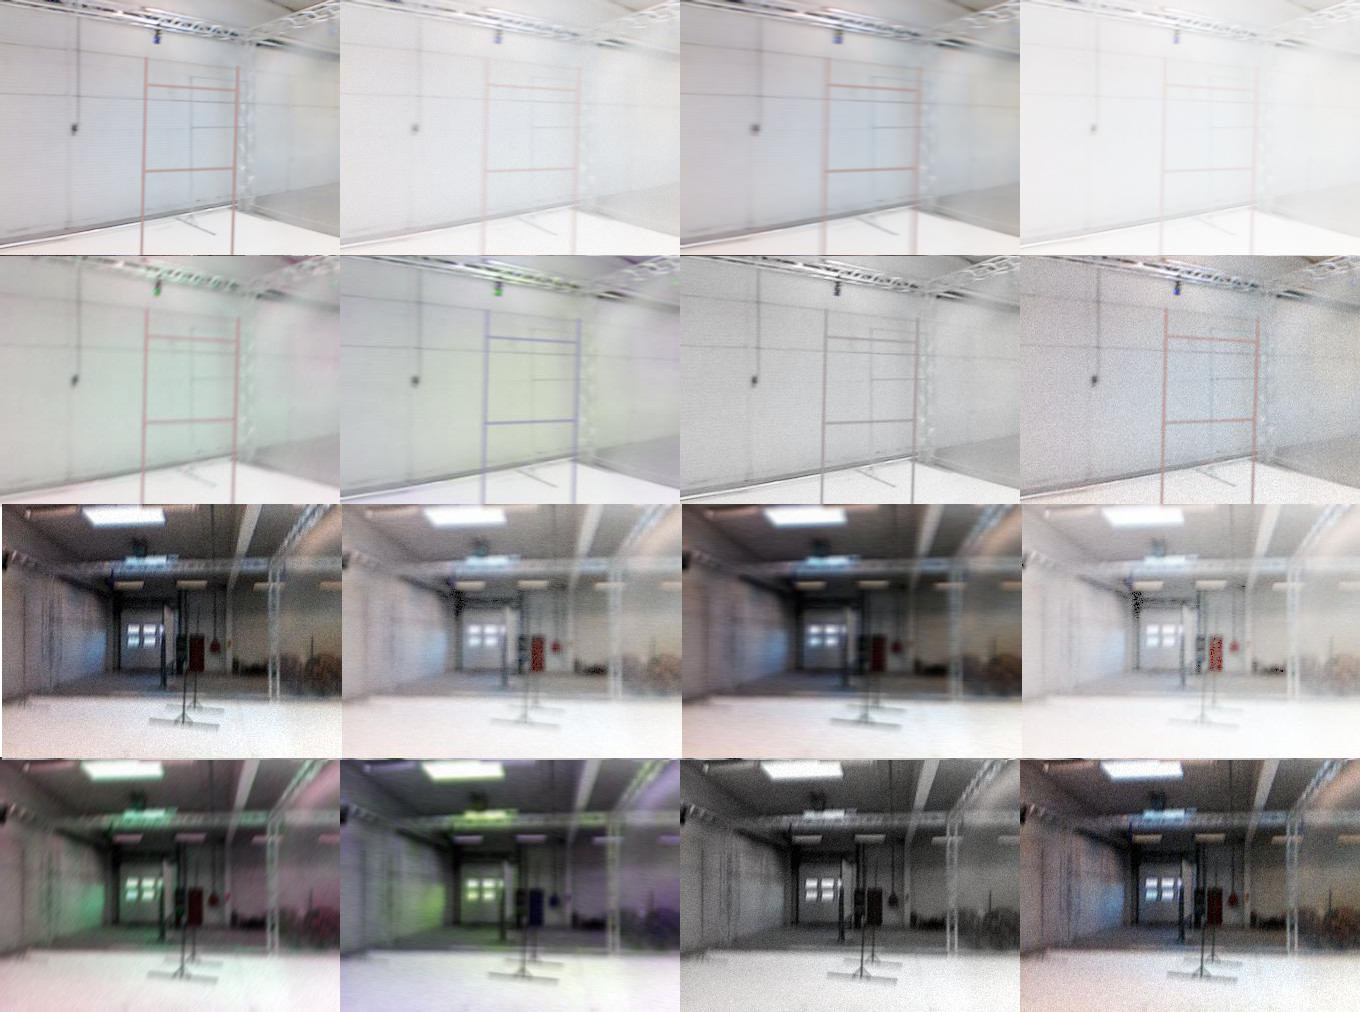
\includegraphics[width=\textwidth]{figure/augmentation.jpg}
    \caption{Few samples of random image transformations applied to one batch.}
    \label{fig:augmentation}
\end{figure}

The effect of applying the said augmentations to the dataset can be seen in
Fig.~\ref{plot:mobilenetv2-aug}, where each plot compares the augmentation
results to their base counterpart. An interesting phenomenon that is visible on
every plot, is the drastic reduction in fluctuation of the validation loss and
accuracy. This can be explained by the fact that the network gets slightly
altered versions of the input at each iteration, and is therefore able to
generalize slightly better. As for the performance of the model, it is visible
that the overfitting is reduced, especially in
Fig.~\ref{plot:mobilenetv2-aug-val-large} where the optimal model topology
minimizes with a constantly positive rate when trained on the augmented
training set.\\

Providing the network with more data, and most importantly with more noisy
samples, has led to a more robust model that is able to generalize better, and
overall give more accurate predictions.

\begin{figure}[h!]
	\centering
	\begin{subfigure}{0.49\textwidth}
		\begin{tikzpicture}
			\pgfplotsset{
				scale only axis,
				legend pos=north east,
				legend entries={No augmentation,Augmentation},
				grid style={dotted,gray,line width=.1pt},
				grid=both
			}
			\begin{axis}[xlabel=Epoch,ylabel=Validation loss,width=7cm,height=7cm]
				\addplot+[mark=none,smooth] table [y=val_loss,col sep=comma]
				{plots/mobilenetv2/mobilenetv2_rgb_hidden_dropout_50000.txt};
				\addplot+[mark=none,smooth] table [y=val_loss,col sep=comma]
				{plots/mobilenetv2/mobilenetv2_rgb_hidden_dropout_aug_50000.txt};
			\end{axis}
		\end{tikzpicture}
		\caption{MobileNetV2 with a hidden layer and dropout on 50,000 samples.}
	\end{subfigure}
	\begin{subfigure}{0.49\textwidth}
		\begin{tikzpicture}
			\pgfplotsset{
				scale only axis,
				legend pos=north east,
				legend entries={No augmentation,Augmentation},
				grid style={dotted,gray,line width=.1pt},
				grid=both
			}
			\begin{axis}[xlabel=Epoch,ylabel=Validation loss,width=7cm,height=7cm]
				\addplot+[mark=none,smooth] table [y=val_loss,col sep=comma]
				{plots/mobilenetv2/mobilenetv2_rgb_avg_pooling_50000.txt};
				\addplot+[mark=none,smooth] table [y=val_loss,col sep=comma]
				{plots/mobilenetv2/mobilenetv2_rgb_avg_pooling_aug_50000.txt};
			\end{axis}
		\end{tikzpicture}
		\caption{MobileNetV2 with average pooling on 50,000 samples.}
	\end{subfigure}

	\begin{subfigure}{0.49\textwidth}
		\begin{tikzpicture}
			\pgfplotsset{
				scale only axis,
				legend pos=north east,
				legend entries={No augmentation,Augmentation},
				grid style={dotted,gray,line width=.1pt},
				grid=both
			}
			\begin{axis}[xlabel=Epoch,ylabel=Validation loss,width=7cm,height=7cm]
				\addplot+[mark=none,smooth] table [y=val_loss,col sep=comma]
				{plots/mobilenetv2/mobilenetv2_rgb_hidden_dropout_avg_pooling_noaug_150000.txt};
				\addplot+[mark=none,smooth] table [y=val_loss,col sep=comma]
				{plots/mobilenetv2/mobilenetv2_rgb_hidden_dropout_avg_pooling_aug_150000.txt};
			\end{axis}
		\end{tikzpicture}
		\caption{MobileNetV2 with a hidden layer, dropout and average pooling
		on 150,000 samples.}
	\end{subfigure}
	\begin{subfigure}{0.49\textwidth}
		\begin{tikzpicture}
			\pgfplotsset{
				scale only axis,
				legend pos=south east,
				legend entries={No augmentation,Augmentation},
				grid style={dotted,gray,line width=.1pt},
				grid=both
			}
			\begin{axis}[xlabel=Epoch,ylabel=Validation accuracy,width=7cm,height=7cm]
				\addplot+[mark=none,smooth] table [y=val_accuracy,col sep=comma]
				{plots/mobilenetv2/mobilenetv2_rgb_hidden_dropout_avg_pooling_noaug_150000.txt};
				\addplot+[mark=none,smooth] table [y=val_accuracy,col sep=comma]
				{plots/mobilenetv2/mobilenetv2_rgb_hidden_dropout_avg_pooling_aug_150000.txt};
			\end{axis}
		\end{tikzpicture}
		\caption{MobileNetV2 with a hidden layer, dropout and average pooling
		on 150,000 samples.}
		\label{plot:mobilenetv2-aug-val-large}
	\end{subfigure}
	\caption{Comparison of MobileNetV2 trained on augmented and original
	datasets.}
	\label{plot:mobilenetv2-aug}
\end{figure}


Most importantly, when evaluated on the real test set, the model showed very
satisfying results that seem to be more accurate than the validation accuracy
would suggest. This makes perfect sense, as the generated dataset contains very
intricate gate configurations which do not represent real world scenarios. This
over-complexification of the problem is an asset that is helpful to train a
robust model. The end result is an alleged gap between test accuracy and
validation accuracy, but in a good way: the model performs better on real
world test data than on synthetic images, supposedly (see
Fig.~\ref{fig:good-test} for more).

To confirm this hypothesis, a proper test dataset with correct ground truth is
needed. For the time being, the best performing model, depicted in
figure~\ref{plot:mobilenetv2-aug-val-large}, is evaluated on the biased test
set in table~\ref{table:mobilenetv2-best}. What stands out from those result is
the accuracy of the model on the real test set, significantly higher than the
previous experiment on table~\ref{table:mobilenetv2-noaug}. The difference
between the top 1 and top 2 accuracies is quite high, reflecting the generally
good performance of the network, considering that this test set contains
wrong ground truth labels in majority. Finally, the top 5 accuracy of the model
on each test set is a promising result, and signifies that with proper fine
tuning of the network, a close-to-perfect accuracy is considered possible.

\begin{table}[!h]
    \centering
    \caption[Top-N accuracies for MobileNetV2 on real and synthetic test
    datasets, with image augmentation]{MobileNetV2 with a hidden layer and
    dropout, coupled with average pooling, trained on 150,000 RGB augmented
    samples, and evaluated on synthetic and real test datasets.}
    \begin{tabular}{llllll}
        \toprule
		Dataset & Top 1 [\%] & Top 2 [\%] & Top 3 [\%] & Top 4 [\%] & Top 5 [\%]\\
        \midrule         
        Synthetic & \textbf{82} & \textbf{91} & \textbf{94} & \textbf{96} &
        \textbf{97} \\ 
        Real & \textbf{45} & \textbf{64} & \textbf{72} & \textbf{76} &
        \textbf{79} \\
        \bottomrule
    \end{tabular}
    \label{table:mobilenetv2-best}
\end{table}


\begin{figure}[h]
    \centering
    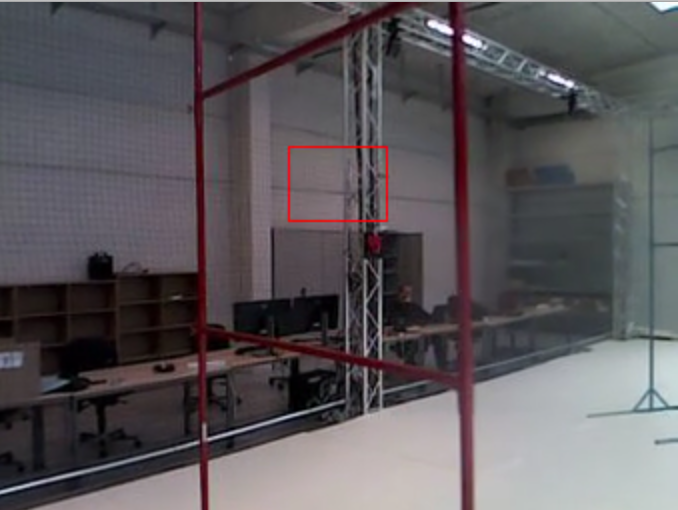
\includegraphics[width=0.7\textwidth]{figure/good_test_res.png}
    \caption[MobileNetV2 showing decent results]{MobileNetV2 showing decent
    predictions with 49 windows on the real test set (see
    https://youtu.be/-cDspgkhHe0 for more).}
    \label{fig:good-test}
\end{figure}
